
\section{Ejercicio 2.}

La red de este ejercicio trata de una comunidad de delfines de Doubtful Sound, Nueva Zelanda. La comunidad, que se constituye de 62 ejemplares identificados por una marca en la aleta dorsal, fue fotografiada entre 1995 y 2001. A partir de esos datos se construyó la red que contiene 159 links, donde se establece que existe un link entre aquellos individuos que fueron vistos juntos de forma más frecuente que la esperada aleatoriamente, es decir, por un criterio de ``compañía preferida".[D. Lusseau, The emergent properties of a dolphin social network, Proc. R. Soc. London B (suppl.) 270, S186-S188 (2003).]

\subsection{Parte a.}

\par Exploramos diferentes layouts para visualizar la red delfines.
En la figura \ref{fig:Layout_delfines} observamos el resultado de graficar
el grafo con el Fruchterman - Reingold layout. El algoritmo para realizar este layout se basa en asignarles fuerzas de interacción ficticias a los nodos. Típicamente se basa en que los nodos ligados tengan una fuerza de atracción análoga a la fuerza de un resorte, sumado a una fuerza de repulsión entre todos los nodos, análoga a la interacción coloumbiana entre partículas cargadas idénticamente. Este tipo de layout nos permitió visualizar la existencia de dos comunas de delfines, ligadas a través de unos pocos nodos.
\par Otros layouts que nos aportarían la misma conclusión son el DrL layout y el Kamada Kawai (fig. \ref{fig:Layouts_alternativos}), que también están basados en la asignación de fuerzas ficticias. Preferimos el Fruchterman - Reingold layout, ya que los nodos aparecen mejor distribuidos, y permite una mejor visualización de la red.
\par A modo de ejemplo, incluímos otros layouts, Random, que sitúa los nodos en forma aleatoria, y Multidimensional Scaling, que se basa en una proyección matricial a un espacio de baja dimensionalidad, que no nos aportaron una buena visualización.

\begin{figure}[h]
\centering
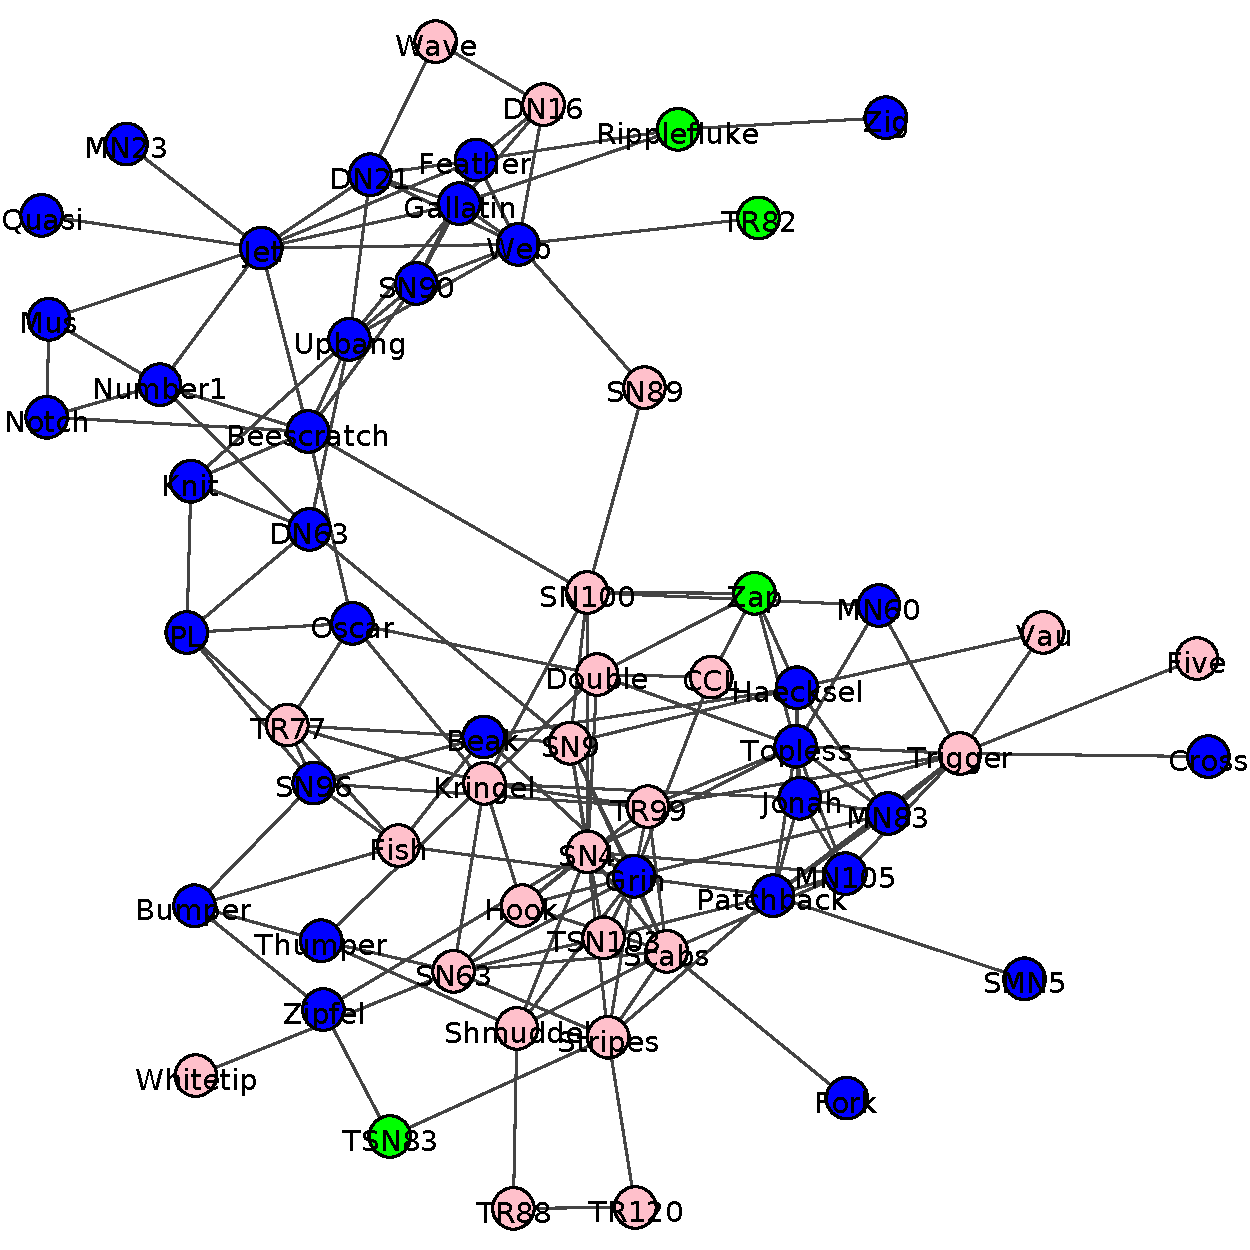
\includegraphics[scale = 0.50]{figuras/FrutRein}
\label{fig:Layout_delfines}
\caption{Fruchterman - Reingold layout. Los colores de los nodos se refieren al sexo del delfín: azul, macho; rosa, hembra; verde, sexo no indicado en el dataset.}
\end{figure}

\begin{figure}[h]
\centering
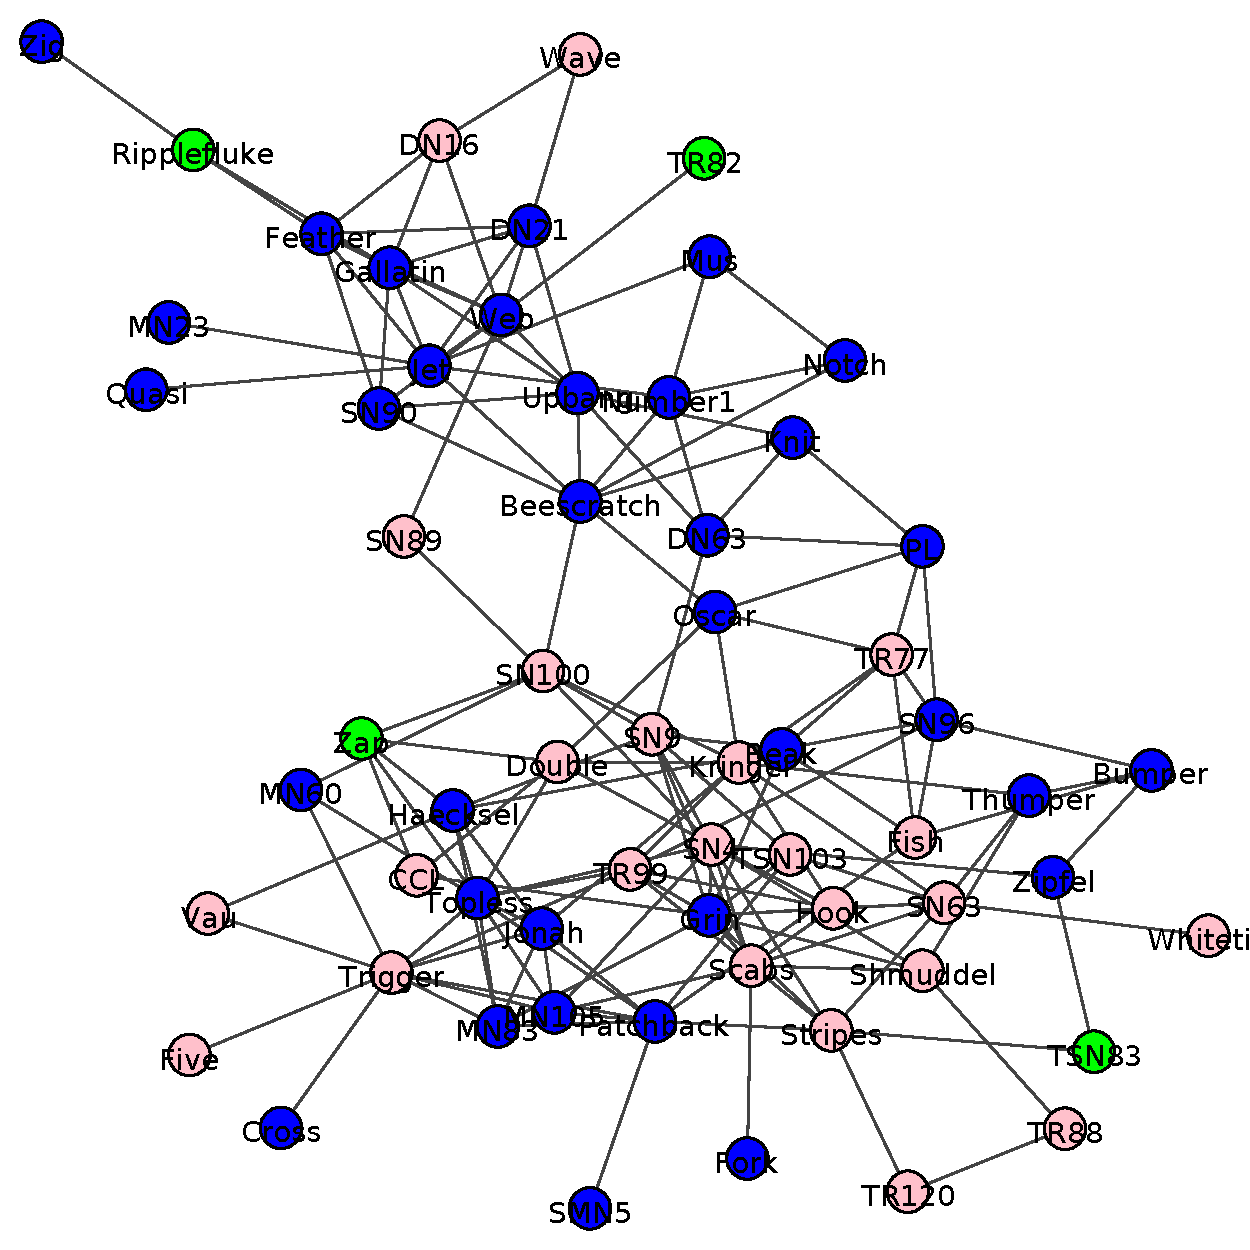
\includegraphics[scale = 0.25]{figuras/KamKaw}
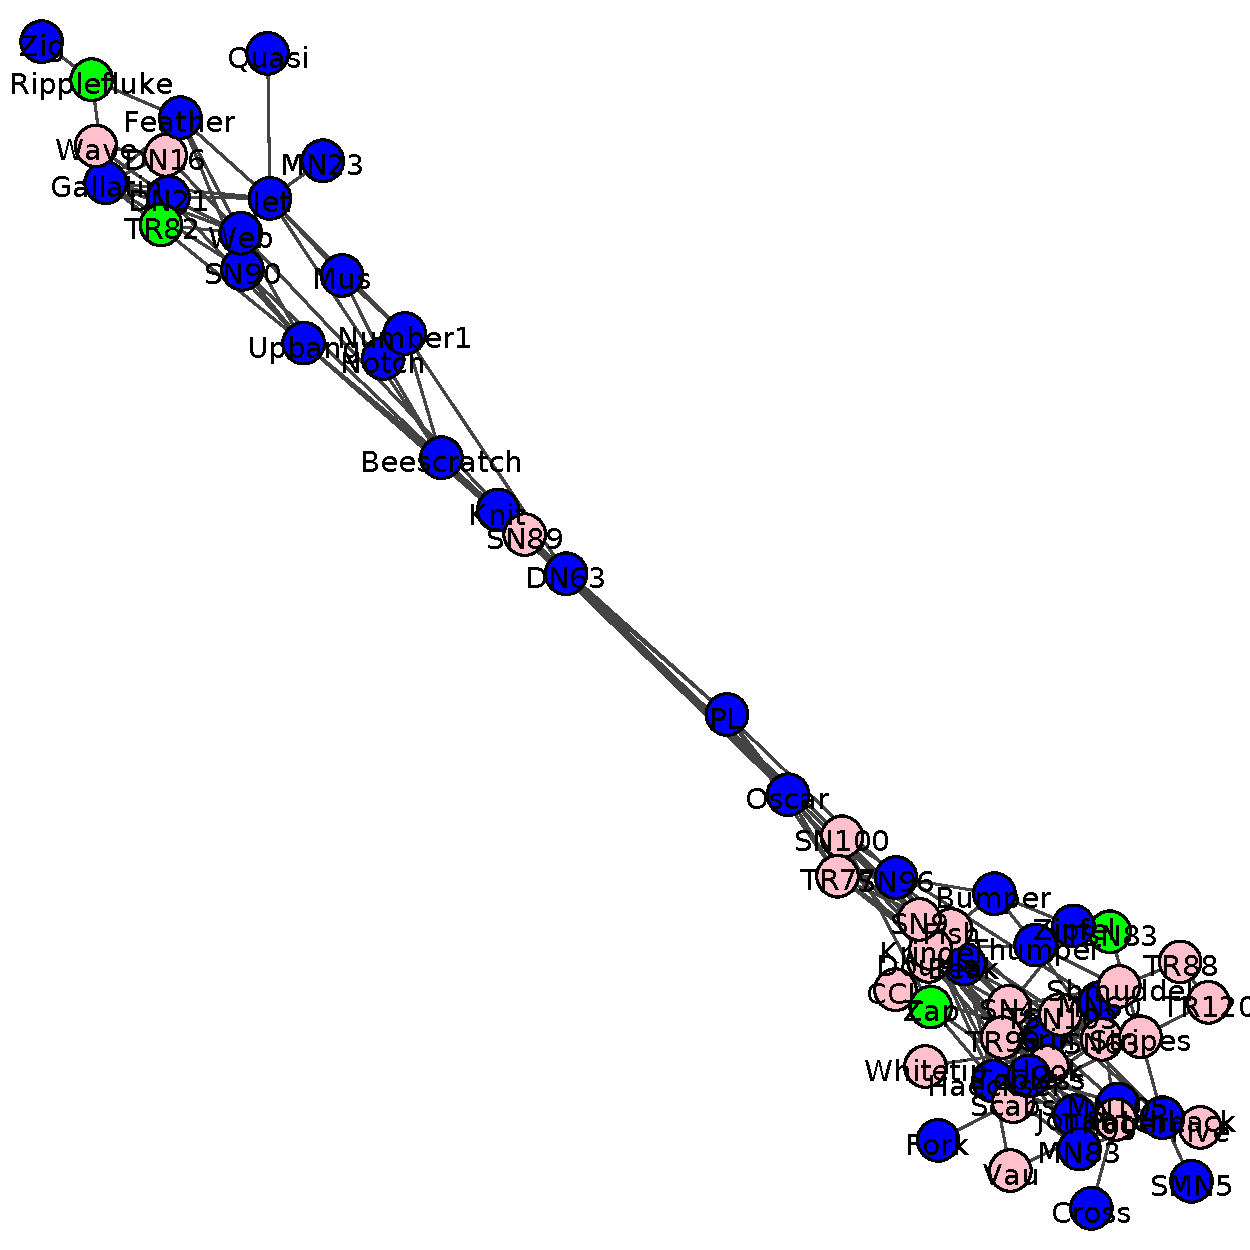
\includegraphics[scale = 0.25]{figuras/Drl}
\label{fig:Layout_alternativos}
\caption{Fruchterman - Reingold layout. Los colores de los nodos se refieren al sexo del delfín: azul, macho; rosa, hembra; verde, sexo no indicado en el dataset.}
\end{figure}

\begin{figure}[h]
\centering
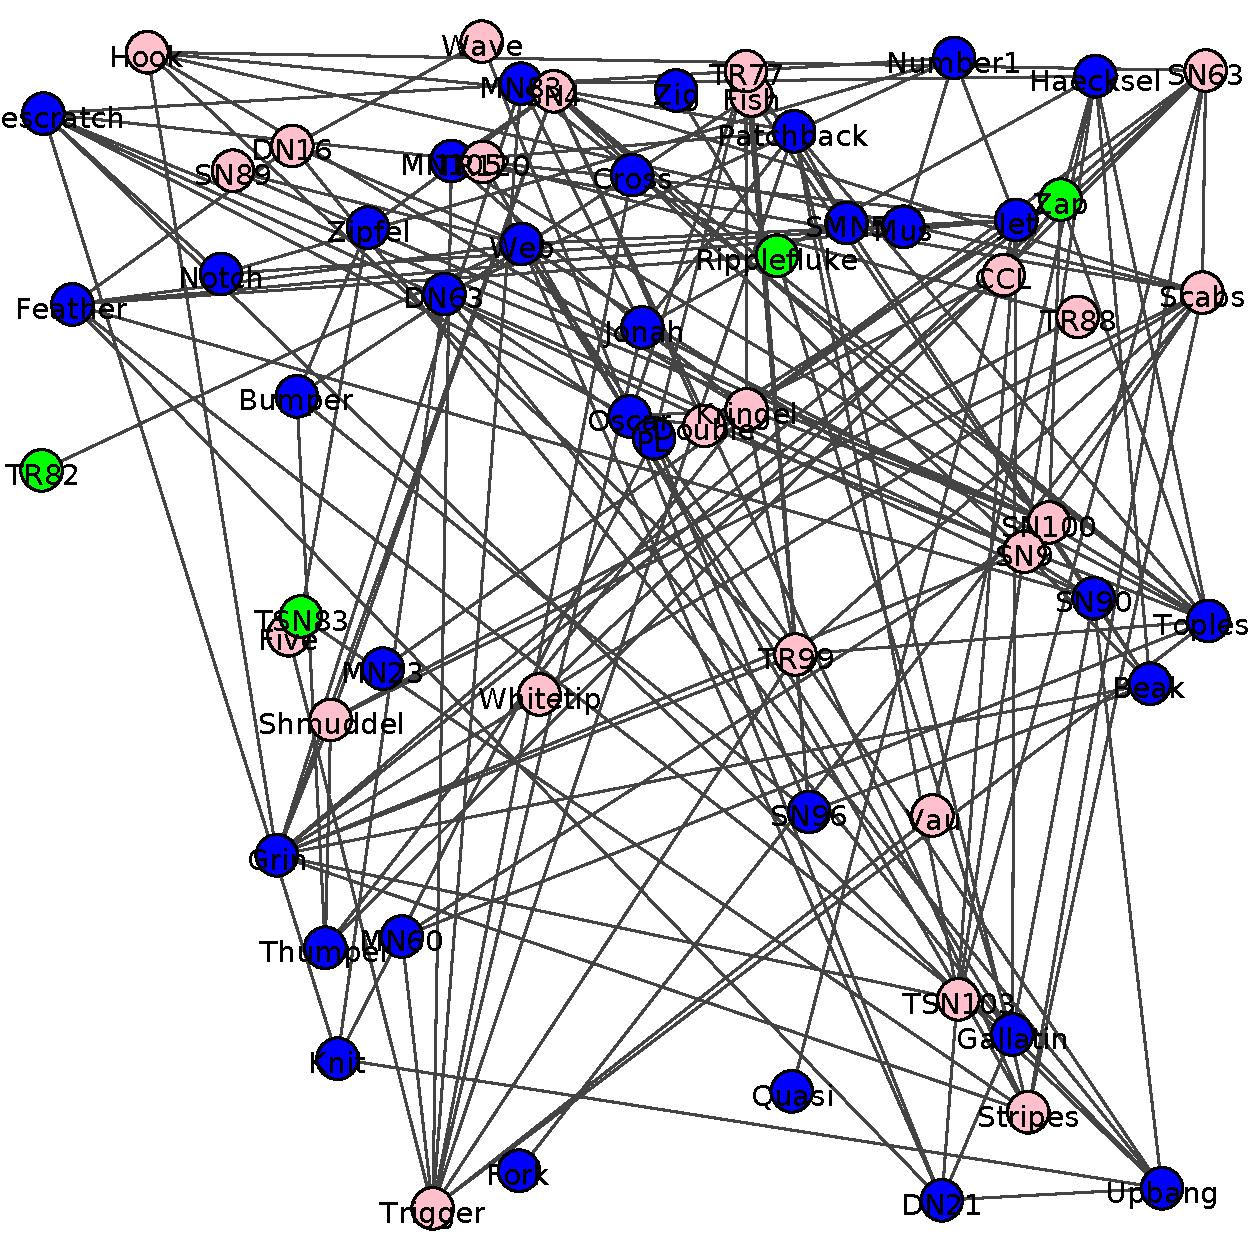
\includegraphics[scale = 0.25]{figuras/Random}
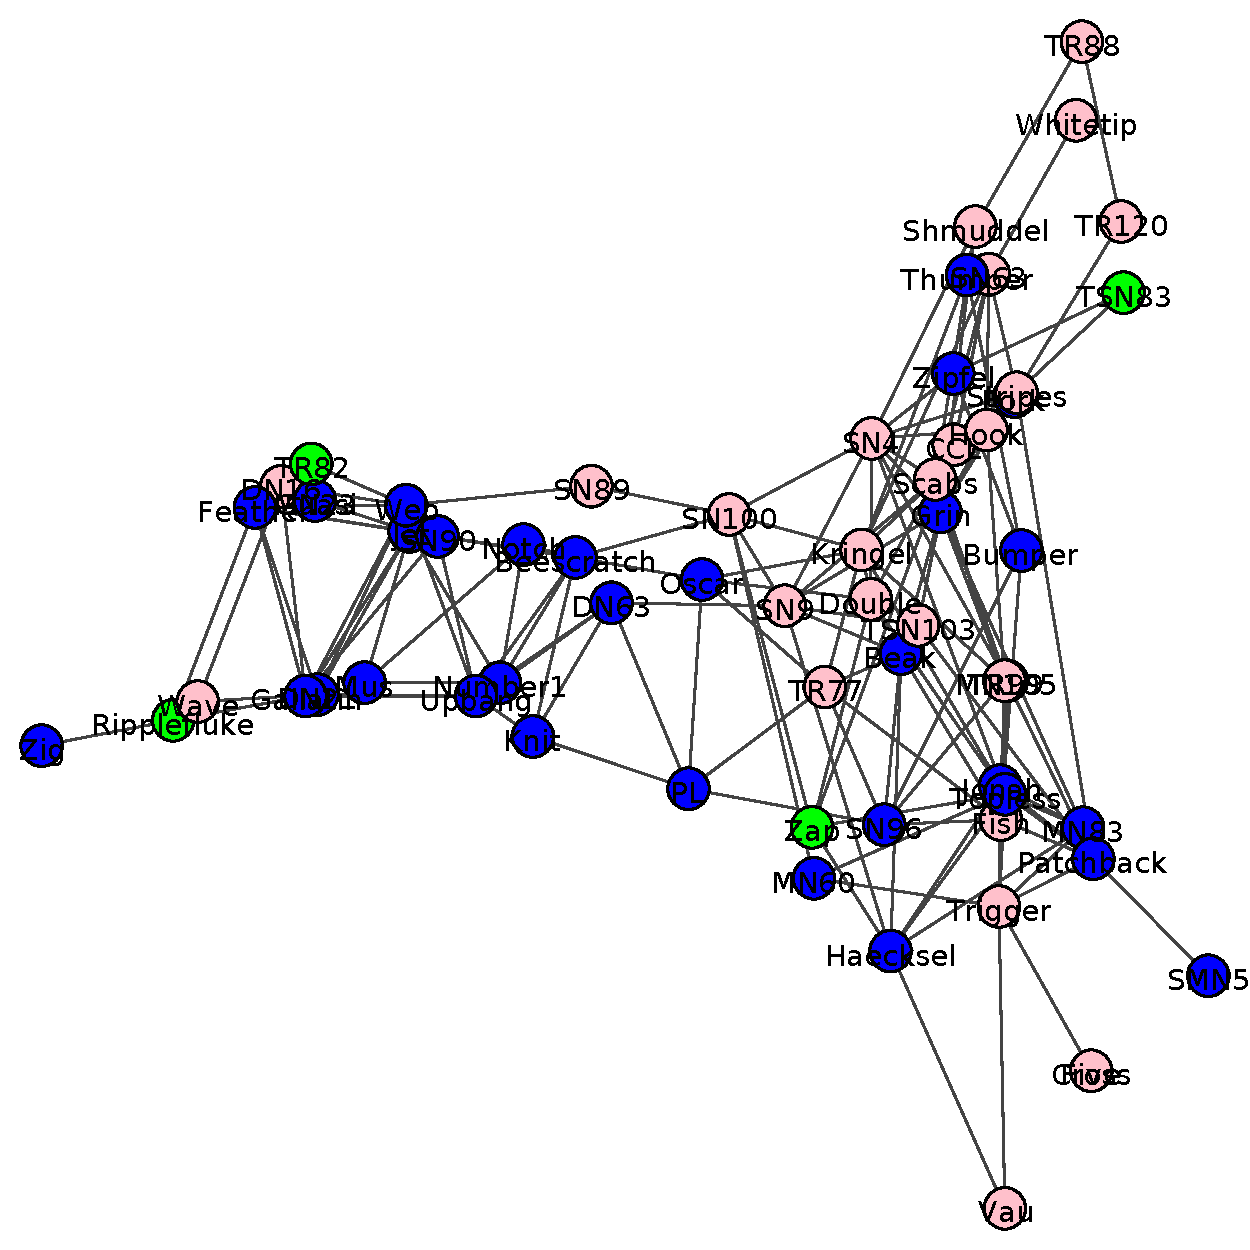
\includegraphics[scale = 0.25]{figuras/Multi}
\label{fig:Layout_malos}
\caption{Fruchterman - Reingold layout. Los colores de los nodos se refieren al sexo del delfín: azul, macho; rosa, hembra; verde, sexo no indicado en el dataset.}
\end{figure}


\subsection{Parte b.}

\par En esta sección nos propusimos estudiar si la red es de carácter homofílica, es decir, si un dado nodo tiende a ligarse con nodos que comparten una característica con él, como es en este caso el género de los delfines. Para ello consideremos la hipótesis nula, es decir, que la asignación de género a un dado nodo es totalmente independiente de la topología de la red, y comparamos con lo presente en el dataset.
\par La metodología empleada fue la siguiente: sorteamos el género de los delfines manteniendo inalterable la topología de la red y manteniendo constante la cantidad de delfines machos, hembras, y género no específicado de la red original. Generamos $10^{6}$ realizaciones distintas, y para cada caso calculamos la cantidad de links entre delfines de distinto género (sin tomar en cuenta los links entre pares de nodos que incluya un género indefinido). El resultado es la distribución de la figura \ref{fig:Histograma}. En el mismo incluímos la cantidad de links entre géneros de la red real, que en principio se observa mucho menor que la media de la distribución.

\begin{figure}[h]
\centering
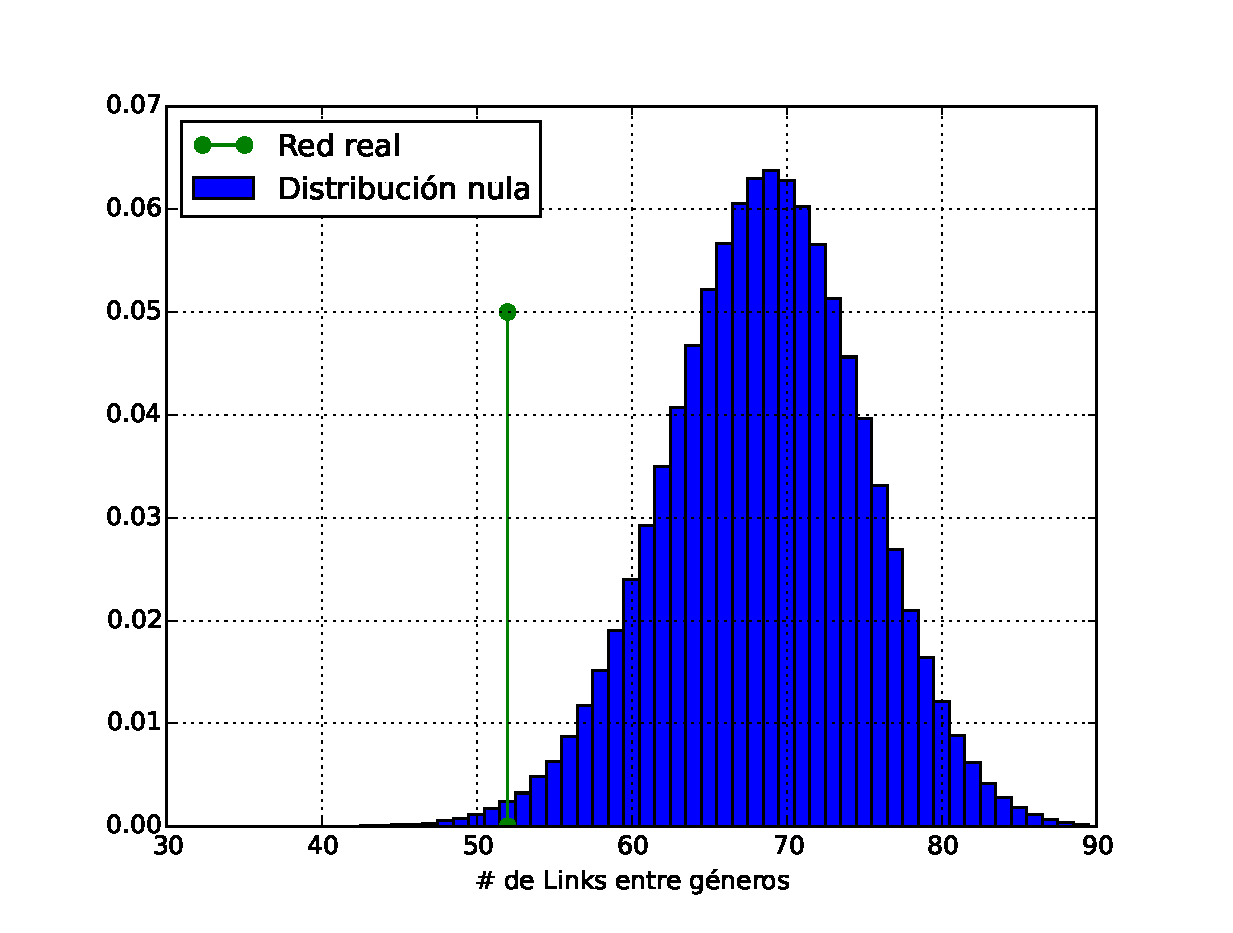
\includegraphics[scale = 0.50]{figuras/Histograma}
\label{fig:Histograma}
\caption{Histograma}
\end{figure}

\par Por otro lado podemos estimar la fracción de links entre géneros para una red aleatoria. Si tomamos que la probabilidad de escoger un link entre un macho y una hembra es $2 \rho_{M} \rho_{F}$, donde $\rho$ son las densidades de cada género en la red real, entonces la probabilidad de la tomar $m$ links de esta característica es:
\begin{equation}
	P(m) = {N' \choose m} (2 \rho_{M} \rho_{F})^{m} (1 - 2 \rho_{M} \rho_{F})^{N' - m}
\end{equation}
donde $N'$ es $N(N-1)/2$, el número total de links que se pueden formar en una red de $N$ nodos. Con esta distribución, el valor medio de links y la desviación standard resultan:
\begin{align*}
	<m> & = 2 N' \rho_{M} \rho_{F} \\
	std(m) & = (2 N' \rho_{M} \rho_{F} (1 - 2 \rho_{M} \rho_{F}))^{1/2}\\
\end{align*}
Por lo tanto, la fracción de links ($<m>/N'$) para las densidades de género actuales, estimado mediante la ecuación anterior, y el resultado del sorteo considerando la hipótesis nula resultan:

\begin{align*}
	(<m>/N')_{estimado} & = 0.43 \pm 0.01 \\
	(<m>/N')_{hip.nula} & = 0.43 \pm 0.04
\end{align*}
donde el último valor se obtuvo dividiendo $<m> = 68 \pm 7$ (obtenido del sorteo) y $N' = 159$, que es el número de links totales de la red real). Observamos que el valor estimado y el obtenido sorteando al azar el género de los delfines coindicen.
\par Como puede deducirse de la figura \ref{fig:Histograma}, la probabilidad de que se obtengan la cantidad de links entre géneros de la red actual dada la hipótesis nula es menor a $0.005$, por lo que descartamos la hipótesis nula, y concluimos que la red es homofílica: la cantidad de links entre géneros es mucho menor que el valor esperado si la distribución de géneros fuera aleatoria, lo que implica que hay más cantidad de enlaces entre delfines del mismo sexo, y además la probabilidad que el valor actual se dé por simple aleatoriedad es muy baja.

\subsection{Parte c.}

\begin{figure}
\centering
\begin{subfloat}[]
{
	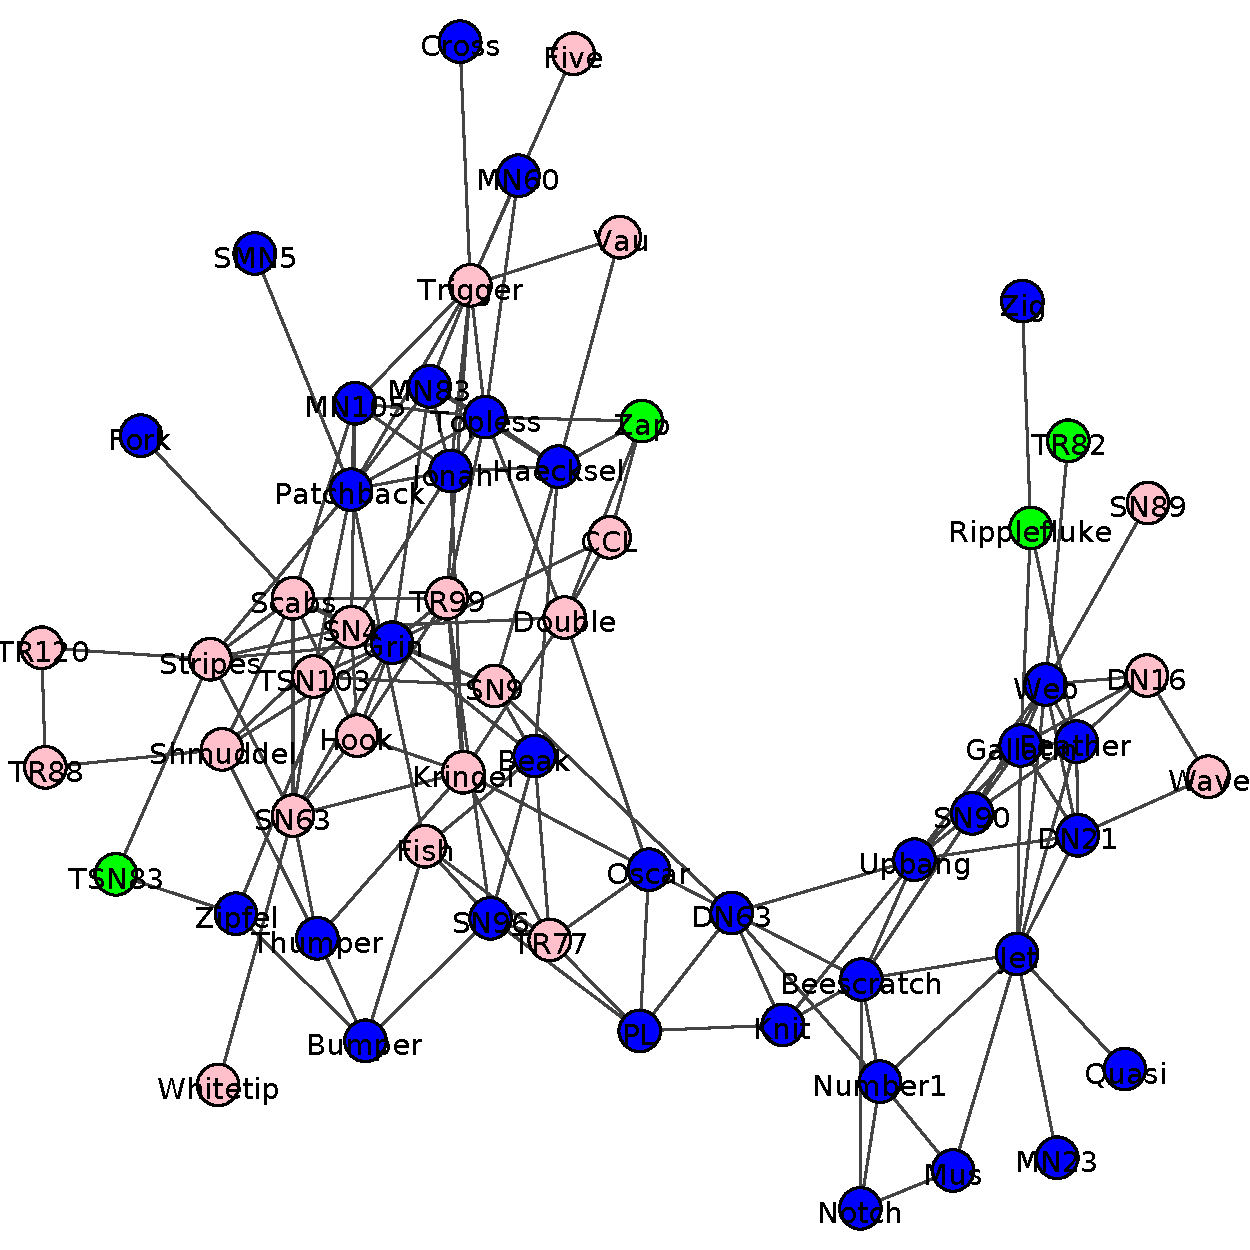
\includegraphics[scale = 0.27]{figuras/Parte_c0} 
}
\end{subfloat}
\begin{subfloat}[]
{
	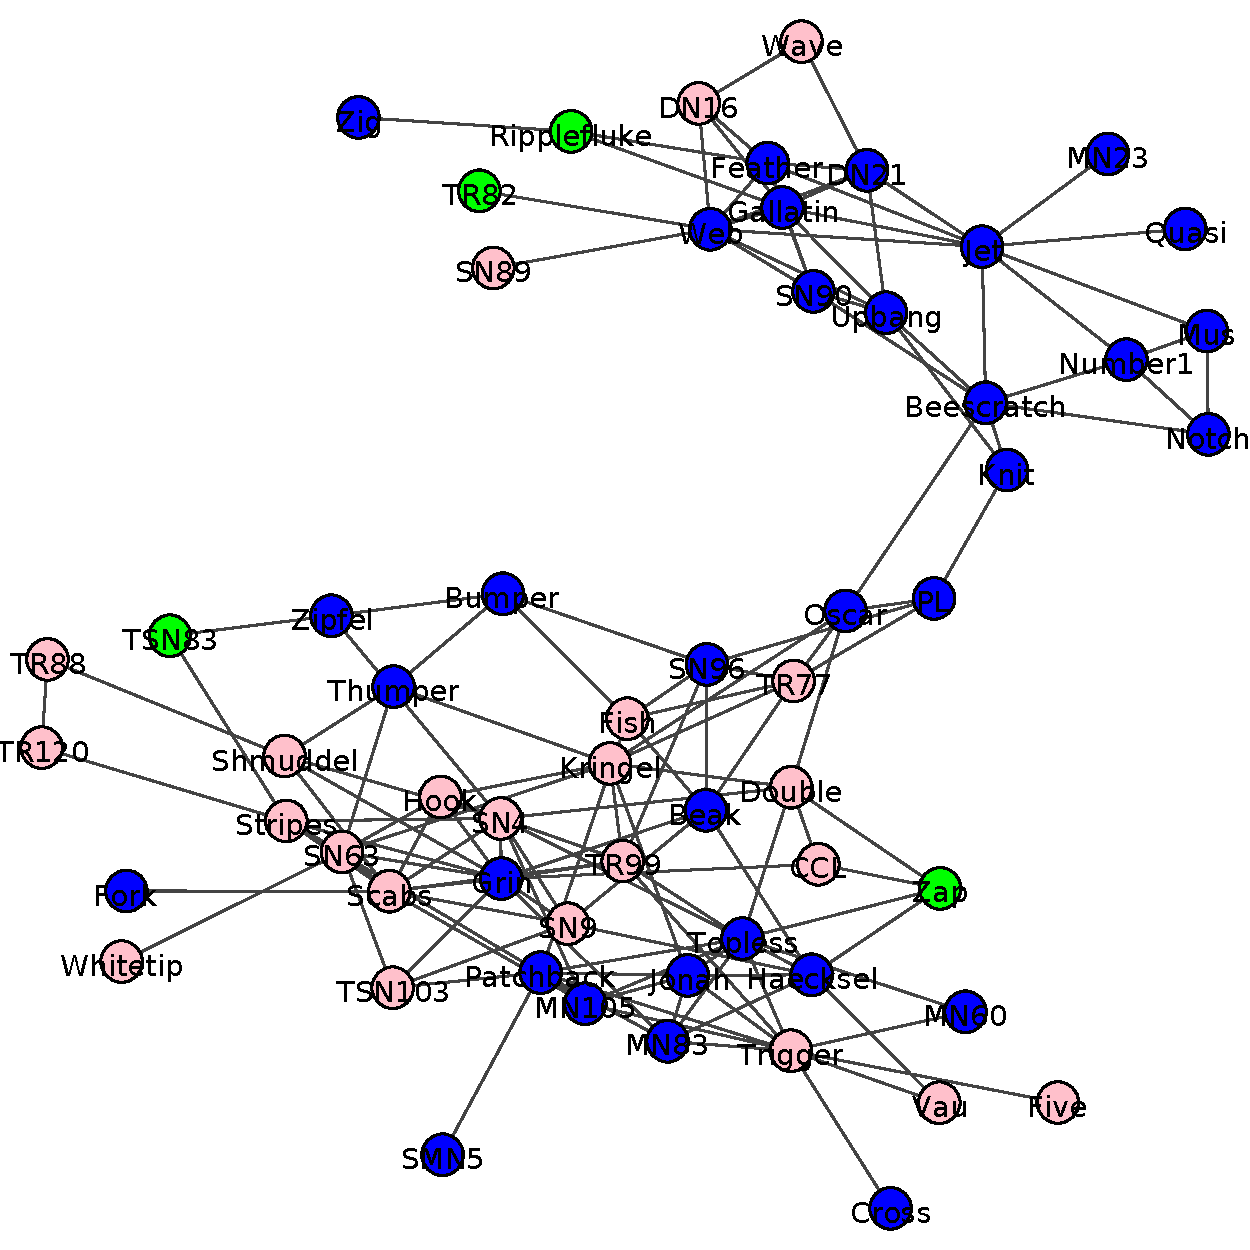
\includegraphics[scale = 0.27]{figuras/Parte_c1}
}
\end{subfloat}
\begin{subfloat}[]
{
	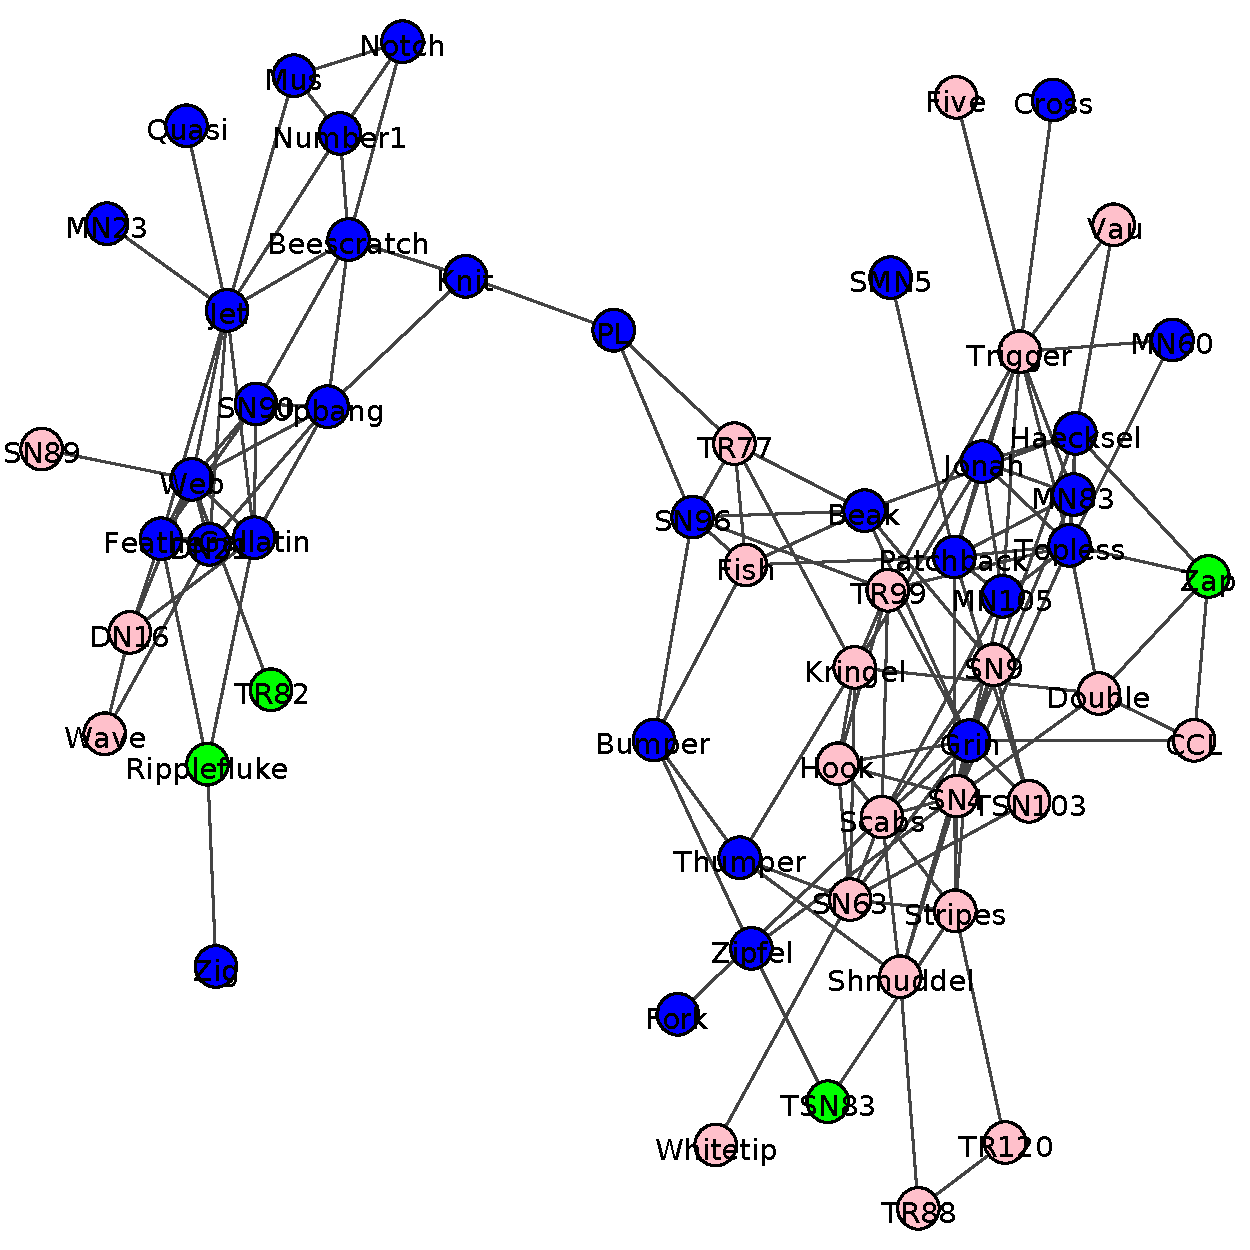
\includegraphics[scale = 0.27]{figuras/Parte_c2} 
}
\end{subfloat}
\begin{subfloat}[]
{
	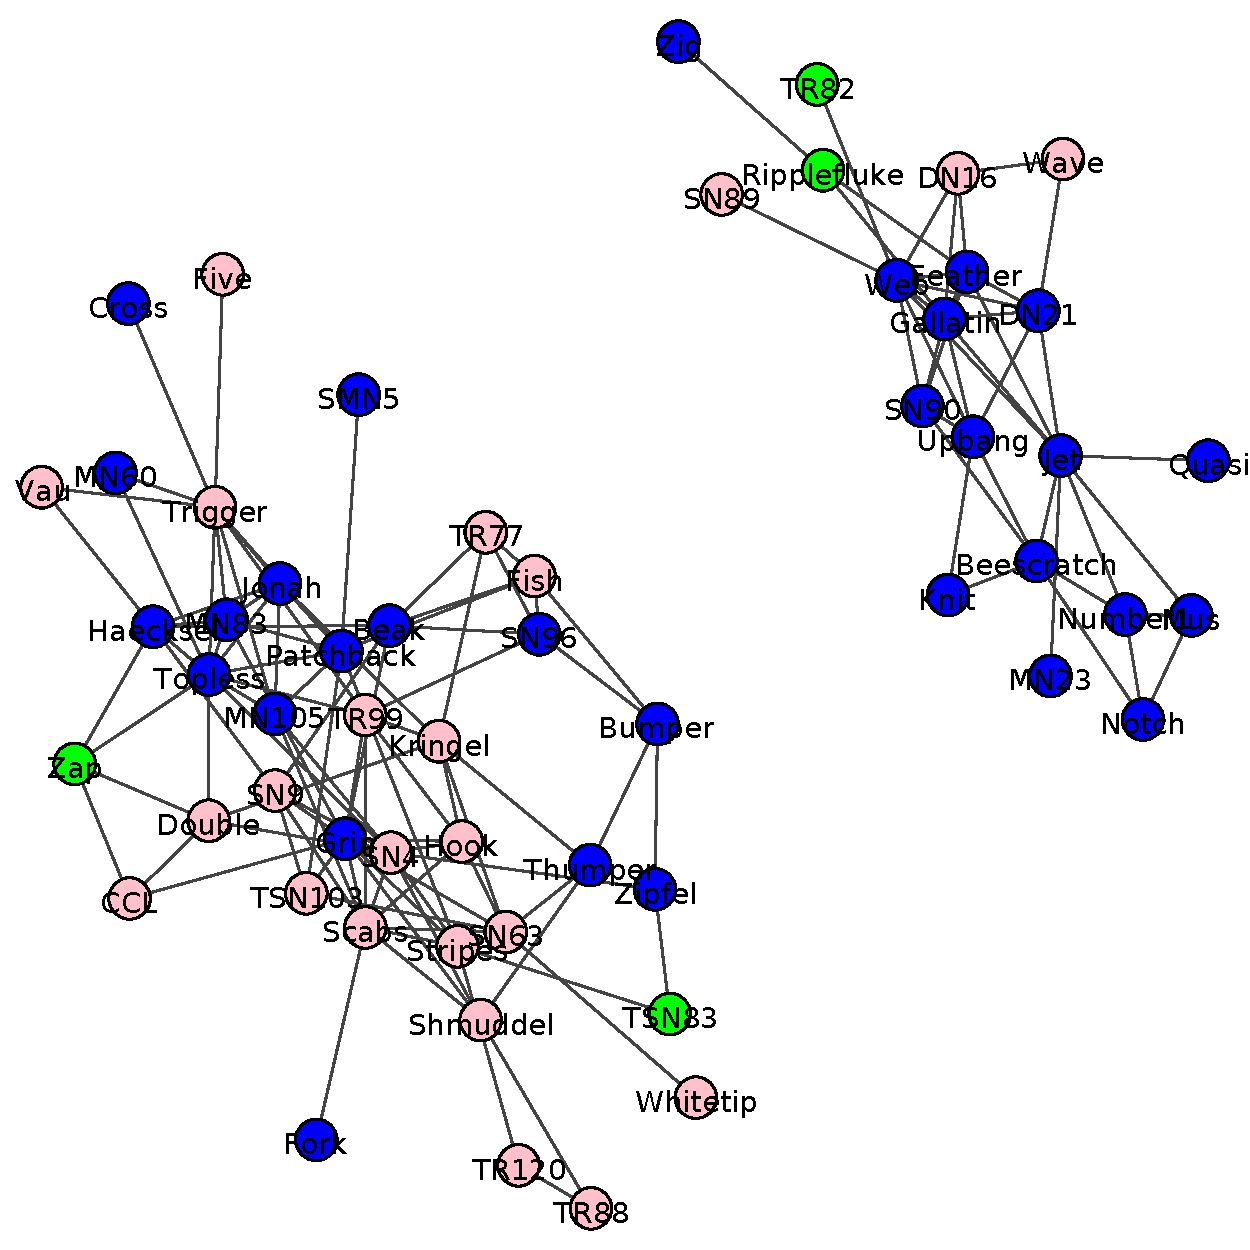
\includegraphics[scale = 0.27]{figuras/Parte_c3} 
}
\end{subfloat}
\label{fig:Betweennes}
\caption{Fruchterman - Reingold layout. Los colores de los nodos se refieren al sexo del delfín: azul, macho; rosa, hembra; verde, sexo no indicado en el dataset.}
\end{figure}
